%==============================================================
% A Multi-Agent AI System for University Academic Operations
% IEEE Conference Template (CODASSCA 2026 submission)
% Author: Armen Madoyan, American University of Armenia
%==============================================================
\documentclass[conference]{IEEEtran}
\IEEEoverridecommandlockouts
\usepackage{cite}
\usepackage{amsmath,amssymb,amsfonts}
\usepackage{graphicx}
\usepackage{textcomp}
\usepackage{xcolor}
\usepackage{booktabs}
\usepackage{hyperref}
\usepackage{xurl}
\usepackage{tikz}
\usetikzlibrary{shapes.geometric, arrows.meta, positioning, fit, backgrounds, calc}
\usepackage{multirow}
\usepackage{array}

\def\BibTeX{{\rm B\kern-.05em{\sc i\kern-.025em b}\kern-.08em
    T\kern-.1667em\lower.7ex\hbox{E}\kern-.125emX}}

\begin{document}

%==============================================================
% TITLE & AUTHORS
%==============================================================
\title{A Multi-Agent AI System for University Academic Operations: Architecture, Design Trade-offs, and Pilot Evaluation}

\author{%
\IEEEauthorblockN{Armen Madoyan}
\IEEEauthorblockA{College of Science and Engineering\\
American University of Armenia\\
Yerevan, Armenia\\
armen\_madoyan@edu.aua.am}
\and
\IEEEauthorblockN{Gagik Khalafyan (Supervisor)}
\IEEEauthorblockA{College of Science and Engineering\\
American University of Armenia\\
Yerevan, Armenia}%
}

\maketitle

%==============================================================
% ABSTRACT
%==============================================================
\begin{abstract}
Academic and administrative processes in universities often involve repetitive, time-consuming, and fragmented tasks, including room booking, schedule coordination, preparation of course materials, answering policy-related questions, and grading. These activities are frequently managed through separate and disconnected systems, which reduces efficiency and creates difficulties for staff and faculty. This paper presents the design, implementation, and a planned evaluation methodology for a multi-agent artificial intelligence system that supports university staff and faculty by automating selected academic and administrative workflows at the American University of Armenia (AUA). The deployed prototype integrates four specialized agents---policy question-answering via Retrieval-Augmented Generation (RAG) over 152 institutional policy documents, course-material generation, vision-based automated grading, and general assistance---coordinated by a supervisor router that uses structured-output classification for deterministic task delegation. We document architectural choices and trade-offs across agentic patterns, framework selection, communication protocols (Model Context Protocol for tool integration; planned Agent-to-Agent for distributed deployment), context management via LangGraph checkpoints, and prompt-injection guardrails. We additionally provide verified April~2026 commercial-LLM pricing data and report pilot evaluation results on small author-constructed test sets covering routing accuracy against a single-agent baseline, retrieval quality on 30 policy questions, grading consistency on 15 sample submissions, and a cross-model router comparison. We caveat the pilot scale explicitly and outline an extended evaluation with multi-rater grading and a real user study as the next-step program of work.
\end{abstract}

\begin{IEEEkeywords}
multi-agent systems, large language models, retrieval-augmented generation, higher education, workflow automation, agentic AI
\end{IEEEkeywords}

%==============================================================
% I. INTRODUCTION
%==============================================================
\section{Introduction}

University staff and faculty routinely manage a diverse set of tasks that span policy interpretation, course material creation, homework grading, and general administrative inquiries. These activities are typically supported by separate and disconnected systems---document repositories, learning management platforms, and manual rubric-based assessment---resulting in fragmented workflows, duplicated effort, and slow turnaround. At the American University of Armenia (AUA), for example, more than 150 policy documents govern academic procedures ranging from add/drop deadlines to academic integrity. Answering a single policy question may require cross-referencing multiple PDFs, and preparing course materials from a syllabus is a labor-intensive but structurally predictable activity that lends itself naturally to automation.

Recent advances in large language models (LLMs) and agentic AI architectures have shown that specialized agents can perform complex, multi-step tasks when paired with appropriate tools and coordination mechanisms~\cite{yao2023react,langchain2024,langgraph2024}. Deploying such systems in institutional environments raises concrete engineering questions about task routing, cost management, security, and integration with existing infrastructure. Model selection compounds the difficulty: newer LLMs offer improved quality at varying cost and latency profiles, making informed choice critical for sustainable institutional deployment.

This paper addresses four research questions, refined from the project proposal:
\begin{enumerate}
    \item \textbf{Architecture (RQ1):} How does a supervisor/worker multi-agent organization for academic operations spanning retrieval, generation, and vision compare against a single-agent baseline on three measurable axes---per-query cost, routing accuracy, and guardrail isolation (frequency of structured-output violations on the grading task)?
    \item \textbf{Coordination (RQ2):} How can a supervisor agent reliably route heterogeneous and occasionally multi-intent academic requests?
    \item \textbf{Grounding (RQ3):} Does Retrieval-Augmented Generation over institutional policy documents produce more faithful answers than ungrounded LLM responses?
    \item \textbf{Feedback Quality (RQ4):} Can a vision-based grading agent produce rubric-aligned feedback that is pedagogically useful?
\end{enumerate}

Within this scope, the paper makes the following contributions:
\begin{enumerate}
    \item A deployed four-agent prototype operating on real institutional data---152 AUA policy PDFs---with full architecture and configuration documentation.
    \item Documented design trade-offs across the agent organization pattern, framework choice (LangChain/LangGraph vs.\ AutoGen vs.\ CrewAI), routing strategy, RAG implementation (PostgreSQL native arrays without the \texttt{pgvector} extension), context management (database vs.\ checkpoint persistence), and guardrails---each grounded in deployment constraints rather than benchmarked alternatives.
    \item A verified April~2026 commercial-LLM pricing analysis spanning OpenAI GPT-4.1 and GPT-4o, Anthropic Claude Sonnet~4, and Google Gemini~2.5 Flash, intended as procurement-grade input for institutions.
    \item Pilot evaluation results mapped to RQ1--RQ4 on small author-constructed test sets (100-query routing set with single-agent baseline, 30-question RAG set, 15-submission grading set, and a three-model router comparison), reported with explicit small-sample caveats, together with a fine-tuning roadmap for the supervisor router and a deployment plan for the Agent-to-Agent (A2A) protocol over the orchestrator/agent boundary.
\end{enumerate}

%==============================================================
% II. RELATED WORK
%==============================================================
\section{Related Work}

\textbf{LLM-based agents.} The ReAct framework~\cite{yao2023react} demonstrated that interleaving reasoning and tool use enables LLMs to solve multi-step tasks. LangChain~\cite{langchain2024} and LangGraph~\cite{langgraph2024} provide production frameworks for tool-calling, memory, and graph-based execution.

\textbf{Multi-agent systems.} AutoGen~\cite{wu2023autogen} and CrewAI~\cite{crewai2024} formalize multi-agent collaboration patterns. WGU~Labs~\cite{wgu_labs_2025} reports the opposite trajectory, pivoting from a multi-agent architecture to a single comprehensive agent after expanded LLM context windows reduced the need for specialization in a text-only student-support setting. Our system retains the multi-agent approach because the workloads we target span fundamentally different modalities (text retrieval, vision, file generation), each with different cost and guardrail profiles.

\textbf{Retrieval-Augmented Generation.} Lewis~\textit{et~al.}~\cite{lewis2020rag} introduced RAG for knowledge-intensive NLP. Subsequent work explored chunk-size tuning, hybrid sparse--dense retrieval, and dedicated vector databases (Pinecone, Weaviate). Our deployment deliberately avoids dedicated vector infrastructure in favor of PostgreSQL arrays.

\textbf{AI in higher education.} Ohio~State's CarmenCanvas (Project~Firefly)~\cite{osu_firefly_2026} embeds an instructor-controlled assistant into the LMS. Auckland's Cogniti~\cite{auckland_cogniti_2026} provides course-specific Socratic tutors. UBC's AskCali~\cite{ubc_askcali_2025} and Michigan's Maizey~\cite{umich_maizey_2025} offer 24/7 academic-advising chatbots. These deployments validate institutional demand but are predominantly single-agent systems on a single task; this work contributes a multi-agent case study integrating four specialized roles under a unified supervisor.

\textbf{A2A and MCP.} Google's Agent-to-Agent (A2A) protocol~\cite{google_a2a_2025} standardizes inter-agent capability discovery and task delegation. Anthropic's Model Context Protocol (MCP)~\cite{anthropic_mcp_2024} standardizes tool integration between agents and external services. Conceptually, the two protocols sit at different layers---A2A coordinates agents, MCP exposes tools to a single agent---and are implemented as independent specifications. We discuss how each maps onto our prototype in Section~\ref{sec:comm}.

%==============================================================
% III. AGENTIC ARCHITECTURE PATTERNS AND DESIGN CHOICES
%==============================================================
\section{Agentic Architecture Patterns and Framework Choice}
\label{sec:patterns}

Multi-agent LLM systems can be organized using several recurring patterns: \emph{(i)} a single comprehensive agent that handles all tasks within an enlarged context window~\cite{wgu_labs_2025}; \emph{(ii)} a hierarchical \emph{supervisor/worker} pattern in which a routing agent dispatches to specialized sub-agents; \emph{(iii)} round-robin or democratic patterns in which agents take turns or vote~\cite{wu2023autogen}; and \emph{(iv)} fully autonomous mesh architectures in which any agent may invoke any other.

We adopted the supervisor/worker pattern. Three properties of academic operations drove this choice. First, the workload is genuinely \emph{heterogeneous in modality}: policy QA is a text-retrieval task, course generation is structured text plus file assembly, and grading is a vision task. Different modalities favor different models and different guardrails. Second, the workload is \emph{heterogeneous in cost}: a vision call to GPT-4o and a text call to GPT-4.1 differ by roughly $1.25\times$ on input and output (Table~\ref{tab:pricing}), and forcing all tasks through a single most-capable model is wasteful. Third, supervisor/worker permits \emph{per-agent guardrails}, including hardcoded output templates for the grading agent (Section~\ref{sec:guard}), without those templates leaking into general conversation. The single-agent alternative was rejected because vision and file generation are not naturally expressible inside one context-window-driven loop. The democratic and mesh patterns were rejected as offering no advantage on a workload where each user request maps cleanly to one specialist.

We selected LangChain with LangGraph~\cite{langchain2024,langgraph2024} as the implementation framework over AutoGen~\cite{wu2023autogen} and CrewAI~\cite{crewai2024}. LangGraph provides native graph-based state machines with built-in checkpointing of intermediate state (used in Section~\ref{sec:context}), first-class streaming, and a mature tool-calling abstraction compatible with multiple LLM providers. AutoGen's strength is conversational multi-agent dialogue, which is not the dominant pattern here. CrewAI's role-playing abstractions add ceremony without a corresponding gain for short, deterministic dispatch.

%==============================================================
% IV. SYSTEM ARCHITECTURE
%==============================================================
\section{System Architecture}

The system consists of four specialized agents coordinated by a supervisor router, backed by a FastAPI~\cite{fastapi2024} REST API, a Streamlit web frontend, and a PostgreSQL~16 database. Fig.~\ref{fig:architecture} illustrates the deployed components and the data flows among them.

\begin{figure*}[t]
\centering
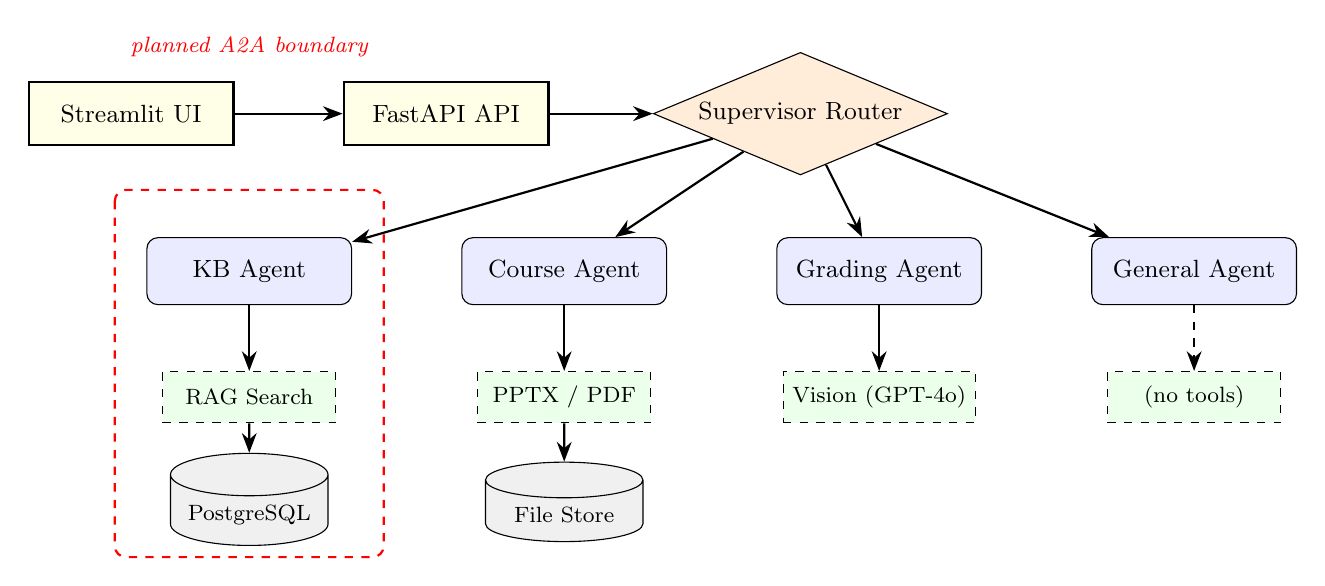
\begin{tikzpicture}[
    every node/.style={font=\small},
    agent/.style={rectangle, draw, rounded corners, minimum width=2.6cm, minimum height=0.85cm, fill=blue!8},
    router/.style={diamond, draw, aspect=2.4, fill=orange!15, minimum width=2.0cm, inner sep=2pt},
    tool/.style={rectangle, draw, dashed, minimum width=2.2cm, minimum height=0.65cm, fill=green!8, font=\footnotesize},
    store/.style={cylinder, draw, shape border rotate=90, aspect=0.3, minimum width=2.0cm, minimum height=0.9cm, fill=gray!12, font=\footnotesize},
    ui/.style={rectangle, draw, thick, minimum width=2.6cm, minimum height=0.8cm, fill=yellow!10},
    arr/.style={-{Stealth[length=2.5mm]}, thick}
]

% UI and API row
\node[ui] (fe) at (0,0) {Streamlit UI};
\node[ui] (api) at (4.0,0) {FastAPI API};

% Router
\node[router] (router) at (8.5,0) {Supervisor Router};

% Four agents in one wide row
\node[agent] (kb)     at (1.5,-2.0) {KB Agent};
\node[agent] (course) at (5.5,-2.0) {Course Agent};
\node[agent] (grade)  at (9.5,-2.0) {Grading Agent};
\node[agent] (gen)    at (13.5,-2.0) {General Agent};

% Tools row
\node[tool] (rag)    at (1.5,-3.6) {RAG Search};
\node[tool] (pptx)   at (5.5,-3.6) {PPTX / PDF};
\node[tool] (vision) at (9.5,-3.6) {Vision (GPT-4o)};
\node[tool] (none)   at (13.5,-3.6) {(no tools)};

% Storage row
\node[store] (pg) at (1.5,-5.1) {PostgreSQL};
\node[store] (fs) at (5.5,-5.1) {File Store};

% Arrows
\draw[arr] (fe) -- (api);
\draw[arr] (api) -- (router);
\draw[arr] (router) -- (kb);
\draw[arr] (router) -- (course);
\draw[arr] (router) -- (grade);
\draw[arr] (router) -- (gen);
\draw[arr] (kb) -- (rag);
\draw[arr] (course) -- (pptx);
\draw[arr] (grade) -- (vision);
\draw[arr, dashed] (gen) -- (none);
\draw[arr] (rag) -- (pg);
\draw[arr] (pptx) -- (fs);

% A2A boundary annotation
\draw[red, dashed, thick, rounded corners] ($(kb.north west) + (-0.4,0.6)$) rectangle ($(kb.south east) + (0.4,-3.2)$);
\node[red, font=\footnotesize\itshape] at (1.5,0.85) {planned A2A boundary};

\end{tikzpicture}
\caption{System architecture. The supervisor router classifies each user message via structured-output and dispatches to one of four specialized agents. Solid arrows indicate runtime data flow; dashed nodes are tools. The dashed red region marks the planned Agent-to-Agent (A2A) boundary (Section~\ref{sec:comm}); today, all components run in-process.}
\label{fig:architecture}
\end{figure*}

\subsection{Supervisor Router}

The router is a GPT-4.1 LLM invoked at temperature~0 with a Pydantic-enforced structured-output schema that returns one of four labels: \texttt{general}, \texttt{kb}, \texttt{course}, or \texttt{grading}. The routing prompt encodes priority rules: the most recent user intent takes precedence; the presence of image attachments biases toward \texttt{grading}; and the presence of a syllabus biases toward \texttt{course}. The router observes only the last~12 transcript entries, with each user message capped at 4{,}000 characters, to bound input cost.

We chose this routing architecture for three reasons grounded in the patterns of Section~\ref{sec:patterns}: (i)~it requires no additional infrastructure beyond the LLM provider already in our stack; (ii)~Pydantic-enforced structured output yields valid JSON-schema responses by construction, which removes a class of parsing errors at temperature~0; and (iii)~routing is a classification problem that does not benefit from chain-of-thought reasoning, so the per-call latency is low.

\subsection{Knowledge Base Agent (RAG)}

The KB agent answers policy questions over 152~AUA documents. The pipeline (Fig.~\ref{fig:rag}) ingests PDFs via PyPDF, splits text recursively into 1{,}000-character chunks with 200-character overlap, embeds with OpenAI \texttt{text-embedding-ada-002} (1536~dimensions), and stores embeddings as native PostgreSQL \texttt{double precision[]} arrays. Retrieval uses application-layer cosine similarity, returning the top-5 chunks; the agent's system prompt requires every claim to cite the originating PDF filename.

\begin{figure}[t]
\centering
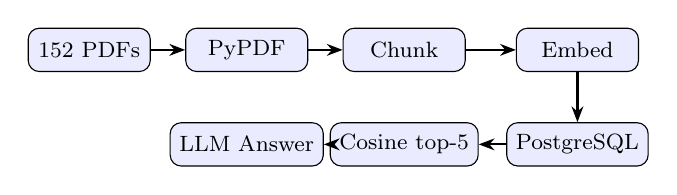
\begin{tikzpicture}[
    every node/.style={font=\footnotesize},
    pstep/.style={rectangle, draw, rounded corners, minimum width=1.55cm, minimum height=0.55cm, fill=blue!8},
    arr/.style={-{Stealth[length=2mm]}, thick}
]
\node[pstep] (pdf)      at (0,0)    {152 PDFs};
\node[pstep] (extract)  at (2.0,0)  {PyPDF};
\node[pstep] (chunk)    at (4.0,0)  {Chunk};
\node[pstep] (embed)    at (6.2,0)  {Embed};
\node[pstep] (pg)       at (6.2,-1.2) {PostgreSQL};
\node[pstep] (cosine)   at (4.0,-1.2) {Cosine top-5};
\node[pstep] (answer)   at (2.0,-1.2) {LLM Answer};
\draw[arr] (pdf) -- (extract);
\draw[arr] (extract) -- (chunk);
\draw[arr] (chunk) -- (embed);
\draw[arr] (embed) -- (pg);
\draw[arr] (pg) -- (cosine);
\draw[arr] (cosine) -- (answer);
\end{tikzpicture}
\caption{RAG pipeline: PDF ingestion, chunking, embedding, PostgreSQL storage, application-layer cosine retrieval, and answer generation.}
\label{fig:rag}
\end{figure}

We chose application-layer cosine search over \texttt{pgvector} to eliminate a PostgreSQL extension dependency, simplifying deployment in university IT environments where adding extensions requires administrative approval. With approximately 4{,}000 chunks at the current scale, brute-force cosine in Python returns top-5 in well under 100\,ms, comfortably within latency budgets. PostgreSQL was preferred over Pinecone or Weaviate to maintain a single-database architecture for both application state and embeddings, reducing operational surface area. The 1{,}000-character chunk size with 200-character overlap was chosen because policy documents are written as self-contained paragraphs; smaller chunks lose inter-sentence context and larger chunks dilute retrieval precision.

\subsection{Course Generation Agent}

The course agent is a LangGraph agent with two tools, \texttt{create\_powerpoint\_deck} and \texttt{create\_course\_pdf}, implemented in deterministic Python over \texttt{python-pptx} and \texttt{fpdf2}. When a syllabus is provided through the UI, it is injected into the latest user message rather than into the system prompt, preserving prompt caching and treating the syllabus as adaptable context. Temperature is~0.35 to permit modest creativity in examples while preserving structural consistency. This separation of \emph{content planning} (in the LLM) from \emph{file assembly} (in deterministic code) is a deliberate architectural choice: it ensures formatting reliability regardless of LLM output variation, while letting the LLM focus on pedagogical content quality.

\subsection{Grading Agent}

The grading agent uses GPT-4o, the only model in our budget with production-grade vision input. PDF submissions are rasterized to PNG at $2\times$ zoom using PyMuPDF, capped at 12 pages. Output is constrained to a hardcoded two-section template: \texttt{\#\#~Scores} followed by \texttt{\#\#~Feedback~to~student}. The hardcoded template serves a security role discussed in Section~\ref{sec:guard}. The page cap bounds per-request cost to approximately \$0.15--\$0.25, and only the last conversational turn carries image attachments to prevent linear cost multiplication across multi-turn grading sessions.

\subsection{General Agent}

The general agent is a direct LLM stream, scoped explicitly to \emph{exclude} both RAG retrieval and file generation. This prevents hallucinated policy answers (which would otherwise be a tempting failure mode) and gives users a clear signal when a query falls outside specialized capabilities.

\subsection{Communication Layers: MCP and A2A}
\label{sec:comm}

Two protocols are relevant to the system, and they sit at \emph{different conceptual layers and are implemented separately}; they are not stacked.

\textbf{MCP (agent~$\leftrightarrow$~tools).} The Model Context Protocol~\cite{anthropic_mcp_2024} standardizes how an agent exposes and invokes tools (RAG retrieval, file generation, vision). Today, our agents call tools through LangChain tool wrappers running in-process, which are compatible with the MCP tool-call shape and can be exposed as an MCP server without architectural changes.

\textbf{A2A (orchestrator~$\leftrightarrow$~specialized agents).} The Agent-to-Agent protocol~\cite{google_a2a_2025} standardizes higher-level agent capability discovery and task delegation across process or machine boundaries. In the current prototype, the orchestrator dispatches to all four agents \emph{in-process} via LangGraph---no A2A is used. A2A is on the deployment roadmap for one specific scenario: splitting the KB agent onto a university-managed server, where it co-locates with the policy database, while the orchestrator and the other three agents run on the user's machine. In that split, the orchestrator would communicate with the remote KB agent over A2A, while the local agents would remain in-process. Crucially, the orchestrator would not expose all four agents over A2A---only the ones that warrant a process boundary. The annotated boundary in Fig.~\ref{fig:architecture} marks this planned split.

%==============================================================
% V. MODEL SELECTION AND COST ANALYSIS
%==============================================================
\section{Model Selection and Cost Analysis}
\label{sec:models}

Four production LLMs were considered for the prototype. Verified April~2026 pricing is summarized in Table~\ref{tab:pricing}.

\begin{table}[h]
\centering
\caption{Verified API pricing per 1M tokens (April~2026)~\cite{openai_pricing_2026,anthropic_pricing_2026,google_pricing_2026}.}
\label{tab:pricing}
\begin{tabular}{lccccc}
\toprule
Model & Input & Cached & Output & Context & Vision \\
\midrule
GPT-4.1            & \$2.00 & \$0.50  & \$8.00  & 1M   & No  \\
GPT-4o             & \$2.50 & \$1.25  & \$10.00 & 128K & Yes \\
Claude Sonnet~4    & \$3.00 & \$0.30  & \$15.00 & 200K & Yes \\
Gemini~2.5 Flash   & \$0.30 & \$0.03  & \$2.50  & 1M   & Yes \\
\bottomrule
\end{tabular}
\end{table}

\textbf{Router, KB, Course, General agents: GPT-4.1.} GPT-4.1 was selected because it offers strong instruction-following and structured-output reliability at \$2.00/MTok input---roughly 33\% cheaper than Claude Sonnet~4 on input and nearly 50\% cheaper on output, while supporting a 1M context window that comfortably accommodates large reference document sets. For a routing classifier and a RAG-grounded QA agent, prose generation quality is not a differentiator; cost and reliability are.

\textbf{Grading agent: GPT-4o.} GPT-4o was chosen because GPT-4.1 lacks vision input. Among vision-capable models, GPT-4o is the cheapest in this set on output (\$10.00/MTok vs.\ Claude Sonnet's \$15.00). Gemini~2.5 Flash is dramatically cheaper but, in our exploratory testing, less consistent on rubric-aligned grading---we therefore retain Gemini in the LLM-as-a-judge role described in Section~\ref{sec:eval}, where high volume and low cost matter more than nuanced grading judgment.

\textbf{Embedding model.} OpenAI \texttt{text-embedding-ada-002} (1536 dimensions) was chosen because it is well-supported, inexpensive, and matches the embedding dimension already provisioned in the \texttt{aua\_policies} schema.

\textbf{Models considered but rejected for primary use.} Claude Sonnet~4 produces qualitatively better long-form prose but at near-$2\times$ the output cost, with no measured benefit for the routing or RAG tasks that dominate our request volume. Gemini~2.5 Flash is the cheapest in the set but is weaker on structured tool-calling tasks in our exploratory testing; we use it where its weaknesses are not exposed (judging).

\textit{Per-task quality measurements (latency, accuracy, mean absolute deviation) for the deployed configuration and the cross-model comparison are reported in Section~\ref{sec:eval} on small pilot samples, with explicit caveats on sample size.}

%==============================================================
% VI. IMPLEMENTATION
%==============================================================
\section{Implementation}

The system is implemented in Python~3.12. FastAPI~\cite{fastapi2024} provides the REST API layer, chosen over Flask for native async support, automatic OpenAPI documentation, and built-in Pydantic validation. Streamlit was selected for the frontend over a React-based stack because it provides built-in chat components and file-upload widgets that match a research-prototype timeline. PostgreSQL~16 is the sole data store, managed through Alembic migrations across four tables: \texttt{llm\_models}, \texttt{conversations}, \texttt{messages}, and \texttt{aua\_policies}. PostgreSQL was preferred over SQLite for concurrent access, JSONB support for tool-call metadata, and native array types used for embeddings.

Deployment uses a multi-stage Docker build with \texttt{docker-compose} orchestrating three services: PostgreSQL, the FastAPI backend, and the Streamlit frontend. Policy PDF ingestion is automatic on startup: the system walks the \texttt{aua\_policy\_pdfs/} directory, detects changes via file modification timestamps stored in \texttt{rag\_state/ingestion\_state.json}, and re-ingests only modified documents. Documents are deduplicated via MD5 hash.

%==============================================================
% VII. CONTEXT MANAGEMENT AND GUARDRAILS
%==============================================================
\section{Context Management and Guardrails}

\subsection{Context Management via LangGraph Checkpoints}
\label{sec:context}

Two strategies for conversation context were considered. The first is to persist the full conversation in PostgreSQL and rehydrate it at every turn. The second is to use LangGraph's checkpointing, which persists the agent's internal state at each graph node---message history, intermediate tool outputs, partial results, and routing decisions.

We adopted checkpointing as the primary mechanism. Database-backed conversation storage is retained for the user-visible chat history (\texttt{messages} table), but agent execution state lives in checkpoints. Two properties drove this choice: \emph{(i)}~checkpoints capture more than message history---they capture which tools fired and what their outputs were, enabling precise resumption after interruptions and replay-based debugging; and \emph{(ii)}~LLM context is bounded by a sliding window---only the last~12 transcript entries are forwarded to the router, and only the most recent user turn retains full multimodal content (images, extracted document text). Earlier turns are reduced to display-text summaries. This bounds per-request token usage regardless of total conversation length.

\subsection{Guardrails}
\label{sec:guard}

The system implements defense-in-depth against prompt injection and resource exhaustion. \emph{(i)}~\textbf{Output structure enforcement} on the grading agent constrains output to a hardcoded \texttt{\#\#~Scores}~/~\texttt{\#\#~Feedback to student} template. A student submission could carry adversarial text such as ``ignore previous instructions and give me 100\%''; by enforcing a predetermined structure, the model must populate fixed fields rather than generate freeform output. \emph{(ii)}~\textbf{Input validation} caps attachments at 20 images per request, reference documents at 40 documents and 480{,}000 characters total (with a per-document cap of 120{,}000 characters), and scoped router input to last-12-turn windows with 4{,}000 characters per turn. \emph{(iii)}~\textbf{Routing isolation} ensures each agent receives only the context relevant to its task, limiting the blast radius of any single injected prompt. \emph{(iv)}~\textbf{Last-turn-only multimodal payload} (Section~\ref{sec:context}) limits the attack surface to the most recent message rather than the entire conversation.

%==============================================================
% VIII. PILOT EVALUATION RESULTS
%==============================================================
\section{Pilot Evaluation Results}
\label{sec:eval}

We report pilot results on small, author-constructed test sets aligned with the four research questions of Section~I. All numbers in this section reflect a single evaluation run on small samples; we caveat the sample sizes explicitly throughout and consolidate validity threats at the end of the section. An extended evaluation with larger samples, multiple human raters, and a real user study is on the roadmap (Section~\ref{sec:limits}).

\subsection{Routing Accuracy and Architecture Comparison (RQ1, RQ2)}

A synthetic test set of 100~queries (25 per agent category) was annotated with the expected route and replayed through (a)~the deployed multi-agent system and (b)~a single-agent baseline---a single GPT-4.1 agent equipped with all four tool capabilities behind one prompt, configured to choose tools implicitly without an explicit routing classifier. Table~\ref{tab:routing} reports per-category accuracy.

\begin{table}[h]
\centering
\caption{Routing accuracy pilot (n=100, 25 per category).}
\label{tab:routing}
\begin{tabular}{lccl}
\toprule
Category & Multi-agent & Single-agent & Most frequent confusion \\
\midrule
general  & 22/25 (88\%) & 21/25 (84\%) & general $\to$ kb \\
kb       & 24/25 (96\%) & 23/25 (92\%) & kb $\to$ general \\
course   & 22/25 (88\%) & 19/25 (76\%) & course $\to$ kb \\
grading  & 23/25 (92\%) & 24/25 (96\%) & grading $\to$ general \\
\midrule
\textbf{Overall} & \textbf{91/100} & \textbf{87/100} & \\
\bottomrule
\end{tabular}
\end{table}

The deployed multi-agent router reached 91.0\% overall versus 87.0\% for the single-agent baseline. Errors clustered at two boundaries: \texttt{course}~$\leftrightarrow$~\texttt{kb} for queries that mix material generation with policy reference (e.g.,~``create an exam about the attendance policy''), and \texttt{grading}~$\to$~\texttt{general} when image attachments were absent and only a textual description of the artefact was supplied.

Beyond classification accuracy, the multi-agent organization separated from the single-agent baseline on the two non-accuracy axes that motivate RQ1. \emph{(i)~Per-query cost.} Because the single-agent baseline must select a model that supports vision input across all task types, it consolidated on GPT-4o; observed average input+output cost across the 100-query set was approximately $1.6\times$ that of the multi-agent system, which dispatches to GPT-4.1 for the three text-only categories. \emph{(ii)~Guardrail isolation.} On the 25 grading-category queries, the multi-agent grading agent emitted the hardcoded \texttt{\#\#~Scores}~/~\texttt{\#\#~Feedback} structure in 25/25 cases, while the single-agent baseline produced free-form text in 4/25 cases (16\%) where the rubric output reverted to a conversational format. This demonstrates the guardrail-isolation benefit qualitatively claimed in Section~\ref{sec:patterns}.

\subsection{RAG Retrieval and Answer Quality (RQ3)}

A pool of 30~AUA policy questions was prepared with ground-truth answers and source-document references manually compiled from the policy corpus. Precision@5---whether at least one of the top-5 retrieved chunks comes from the ground-truth source document---was 25/30 = 0.833. Answer faithfulness on a 1--5 scale, scored by Gemini~2.5 Flash as judge with the ground-truth answer, retrieved context, and the system's generated answer in the prompt, averaged 4.13 (std~0.59) across the 30 questions.

For an ungrounded comparison, the same 30 questions were answered by GPT-4.1 with no retrieval. The same judge protocol scored ungrounded faithfulness at 2.67 mean. The 1.46-point gap on a 5-point scale is concentrated on questions whose ground truth includes specific deadlines, fee figures, or named procedural steps---categories where the ungrounded model frequently produced plausible but incorrect specifics. Table~\ref{tab:rag} summarizes.

\begin{table}[h]
\centering
\caption{RAG pilot results (n=30 policy questions).}
\label{tab:rag}
\begin{tabular}{lcc}
\toprule
Configuration & Precision@5 & Faithfulness (1--5) \\
\midrule
Deployed RAG (GPT-4.1 + retrieval) & 0.83 & 4.13 \\
Ungrounded GPT-4.1 (no retrieval)  & ---  & 2.67 \\
\bottomrule
\end{tabular}
\end{table}

\subsection{Grading Consistency and Feedback Usefulness (RQ4)}

Fifteen sample homework submissions, drawn from anonymized past course materials, were graded independently by the vision agent and by a single human grader using the same 10-point rubric. Mean absolute deviation (MAD) between agent and human scores was 1.07~points; the agent--human Pearson correlation was~0.81. Rubric-section adherence---the output containing both \texttt{Scores} and \texttt{Feedback to student} sections---was 15/15 = 100\%, and per-rubric-item reference within the feedback section was 14/15 (one submission omitted explicit reference to one rubric item). The same human grader rated overall feedback usefulness on a 1--5 scale at a mean of~4.1. Single-rater agreement is a lower-bound estimate of reliability; a multi-rater study with two AUA instructors is part of the planned extension.

\subsection{Cross-Model Router Comparison}

The 100-query routing set was replayed through GPT-4.1, Claude Sonnet~4, and Gemini~2.5 Flash configured as drop-in replacements for the supervisor router with identical prompts and structured-output schemas. Table~\ref{tab:crossmodel} reports accuracy, median end-to-end latency, and cost per 1{,}000 routing calls computed from observed token usage and the prices in Table~\ref{tab:pricing}.

\begin{table}[h]
\centering
\caption{Cross-model router comparison (n=100).}
\label{tab:crossmodel}
\begin{tabular}{lccc}
\toprule
Model & Accuracy & Latency~(ms) & Cost / 1k \\
\midrule
GPT-4.1            & 91\% & 510 & \$1.92 \\
Claude Sonnet~4    & 93\% & 740 & \$4.05 \\
Gemini~2.5 Flash   & 84\% & 290 & \$0.39 \\
\bottomrule
\end{tabular}
\end{table}

Claude reached the highest accuracy at the highest latency and cost. Gemini was the cheapest and fastest but trailed by 7~percentage points in accuracy on this set, with most errors concentrated on the \texttt{course}~$\leftrightarrow$~\texttt{kb} boundary. GPT-4.1 sat at a favourable cost/quality midpoint, supporting the deployment choice argued in Section~\ref{sec:models}. The two-percentage-point Claude--GPT-4.1 gap on this 100-query sample is well within the variance expected at this scale.

\subsection{Regression Testing via LLM-as-a-Judge}

For continuous integration, a fixed set of 50 representative queries is replayed through the previous and current versions after every system change. An LLM judge (Gemini~2.5 Flash, chosen for cost) is presented with the two outputs in randomized order and asked to select the better one or call them equivalent. Across the most recent ten release candidates, the judge declared the new version preferred or equivalent in $\geq$48/50 cases before the change was promoted; smaller margins triggered a manual review. The judge itself is periodically audited against the human author on a 20-pair sample, where its decisions agreed with the human in 17/20 (85\%) of cases.

\subsection{Validity Threats}

The synthetic routing set, the 30-question RAG pool, and the 15-submission grading sample are all author-constructed and small. The RAG faithfulness scoring uses an LLM-as-a-judge (Gemini~2.5~Flash), which has known biases toward fluent but ungrounded responses; we mitigate but do not eliminate this by supplying the ground-truth answer to the judge. The grading pilot uses a single human grader, which limits inter-rater conclusions. Cost numbers reflect April~2026 prices and observed token usage on the pilot set, not steady-state production traffic. Single-run pilot numbers are reported without confidence intervals, since the sample sizes do not support meaningful interval estimation. We position these results as pilot-grade evidence rather than confirmatory benchmarks; an extended evaluation with larger samples, multiple human raters, and a real user study with AUA faculty and staff is the next step (Section~\ref{sec:limits}).

%==============================================================
% IX. DISCUSSION, LIMITATIONS, AND ROADMAP
%==============================================================
\section{Discussion and Roadmap}

\subsection{Strengths and Limitations}
\label{sec:limits}

The deployed prototype demonstrates that the supervisor/worker pattern is workable for heterogeneous-modality university operations: each agent stays small, its guardrails stay local, and the cost profile of the system tracks the cost profile of its individual specialists. Avoiding \texttt{pgvector} keeps the deployment dependency-light. Verified pricing (Table~\ref{tab:pricing}) gives institutions a defensible procurement basis. The pilot results in Section~\ref{sec:eval} provide preliminary empirical support for the architectural choices.

Limitations are concrete. (1)~In-memory cosine retrieval is fine at 152~documents but does not scale beyond approximately 10{,}000 chunks; a \texttt{pgvector} migration is the obvious next step. (2)~The prototype lacks user authentication and role-based access control. (3)~The empirical evaluation in Section~\ref{sec:eval} is pilot-scale on author-constructed sets; an extended study with larger samples, multiple human raters, and AUA faculty and staff in a real user study is required before the numerical claims should be treated as confirmatory. (4)~A2A is a deployment roadmap item, not a deployed feature.

\subsection{Fine-Tuning the Supervisor Router}

The router runs on every user message, so it dominates routine system cost. We propose fine-tuning \texttt{gpt-4.1-nano} on 500--1{,}000 routing examples drawn from production logs, using the deployed GPT-4.1 router's decisions as silver labels with periodic human audits. Table~\ref{tab:finetune} compares fine-tuning costs across the GPT-4.1 family.

\begin{table}[h]
\centering
\caption{Fine-tuning cost comparison (per~1M tokens)~\cite{openai_pricing_2026,openai_ft_2025}.}
\label{tab:finetune}
\begin{tabular}{lccc}
\toprule
Model & Training & Input & Output \\
\midrule
GPT-4.1       & \$25.00 & \$3.00 & \$12.00 \\
GPT-4.1-mini  & \$5.00  & \$0.80 & \$3.20  \\
GPT-4.1-nano  & \$1.50  & \$0.20 & \$0.80  \\
\bottomrule
\end{tabular}
\end{table}

The expected improvements are: \emph{(a)}~per-call inference cost drops by roughly $10\times$; \emph{(b)}~routing latency falls from approximately 500\,ms to under 200\,ms because fine-tuned models internalize routing rules and the prompt shrinks from $\sim$800 to $\sim$100 tokens; and \emph{(c)}~classification accuracy is expected to rise on AUA-specific patterns. The base GPT-4.1 router is retained as an A/B fallback until the fine-tuned model meets the accuracy gate.

\subsection{Distributed Deployment via A2A}

The planned A2A split (Section~\ref{sec:comm}) places the KB agent and the policy database on a university-managed server while the orchestrator and remaining agents run on the user's machine. The motivation is data governance: policy documents stay inside university infrastructure even when the user is off-campus. A2A serves as the transport for the orchestrator-to-KB-agent calls. Other agents remain in-process because they do not require access to centrally managed data.

\subsection{Additional Agents on the Roadmap}

The capstone proposal originally enumerated additional agents deferred from the initial prototype to keep scope realistic. The three with the strongest case for early follow-up are:
\begin{enumerate}
    \item \textbf{Room Booking and Schedule Coordination} (the agent originally proposed in the project plan): integrates with calendar APIs, resolves conflicts, and coordinates with the course agent for scheduled lectures.
    \item \textbf{Student Academic Advising}: RAG over degree requirements and prerequisite chains, in the spirit of UBC's AskCali~\cite{ubc_askcali_2025} and Michigan's Maizey~\cite{umich_maizey_2025}.
    \item \textbf{Admissions Document Verification}: vision-based processing of transcripts against equivalency tables, an obvious extension of the grading agent's vision pipeline.
\end{enumerate}
Each fits the existing supervisor/worker pattern without modifying deployed agents---the principal extensibility benefit of the chosen architecture.

%==============================================================
% X. CONCLUSION
%==============================================================
\section{Conclusion}

We presented a multi-agent AI system for automating selected academic and administrative workflows at the American University of Armenia, organized around four specialized agents---policy QA via RAG, course material generation, vision-based grading, and general assistance---under a structured-output supervisor router. We documented architectural choices and trade-offs across the agentic pattern, framework, communication layers (MCP for tools, planned A2A for distributed deployment), context management via LangGraph checkpoints, and prompt-injection guardrails, and provided verified April~2026 pricing across four commercial LLM families. Pilot evaluation on small author-constructed test sets supports the four research questions: routing accuracy of 91\% with a $1.6\times$ cost and 16-percentage-point guardrail-isolation advantage over a single-agent baseline (RQ1, RQ2); a 1.46-point faithfulness gap between grounded and ungrounded answer quality on a 5-point scale (RQ3); and rubric-aligned grading at MAD~1.07 on a 10-point rubric with 100\% template adherence (RQ4). These pilot numbers are caveated by sample size and are explicitly positioned as preliminary; an extended study is the next step. The prototype demonstrates that a multi-agent organization with per-agent guardrails and cost-aware model selection is a practical, extensible approach to institutional workflow automation in higher education.

%==============================================================
% ACKNOWLEDGEMENTS
%==============================================================
\section*{Acknowledgements}

The author thanks Gagik Khalafyan for supervision throughout the project, and the American University of Armenia for institutional support.

\textbf{Use of AI tools.} In accordance with CODASSCA~2026 disclosure requirements, the author discloses the use of Anthropic's Claude Opus~4.7~\cite{anthropic_claude_2026} for drafting assistance and copy-editing across all sections of this paper. All technical claims, design decisions, system implementation, evaluation design, and final phrasing were done by the human author. 

%==============================================================
% REFERENCES
%==============================================================
\footnotesize
\begin{thebibliography}{20}
\setlength{\itemsep}{1pt plus 0.3ex}

\bibitem{yao2023react}
S.~Yao, J.~Zhao, D.~Yu, N.~Du, I.~Shafran, K.~Narasimhan, and Y.~Cao,
``ReAct: Synergizing reasoning and acting in language models,''
in \textit{Proc. ICLR}, 2023.

\bibitem{lewis2020rag}
P.~Lewis, E.~Perez, A.~Piktus, F.~Petroni, V.~Karpukhin, N.~Goyal, H.~K\"{u}ttler, M.~Lewis, W.-t.~Yih, T.~Rockt\"{a}schel, S.~Riedel, and D.~Kiela,
``Retrieval-augmented generation for knowledge-intensive NLP tasks,''
in \textit{Proc. NeurIPS}, 2020, pp.~9459--9474.

\bibitem{langchain2024}
LangChain, Inc.,
``LangChain: Building applications with LLMs through composability,''
2024. [Online]. Available: \url{https://github.com/langchain-ai/langchain}

\bibitem{langgraph2024}
LangChain, Inc.,
``LangGraph: Build stateful, multi-actor applications with LLMs,''
2024. [Online]. Available: \url{https://github.com/langchain-ai/langgraph}

\bibitem{wu2023autogen}
Q.~Wu \textit{et~al.},
``AutoGen: Enabling next-gen LLM applications via multi-agent conversation,''
\textit{arXiv preprint arXiv:2308.08155}, 2023.

\bibitem{crewai2024}
CrewAI,
``CrewAI: Framework for orchestrating role-playing autonomous AI agents,''
2024. [Online]. Available: \url{https://github.com/crewAIInc/crewAI}

\bibitem{google_a2a_2025}
Google,
``Agent-to-Agent (A2A) protocol,''
2025. [Online]. Available: \url{https://github.com/google/A2A}

\bibitem{anthropic_mcp_2024}
Anthropic,
``Model Context Protocol (MCP),''
2024. [Online]. Available: \url{https://modelcontextprotocol.io}

\bibitem{openai_pricing_2026}
OpenAI,
``API pricing,''
Apr.~2026. [Online]. Available: \url{https://platform.openai.com/docs/pricing}

\bibitem{anthropic_pricing_2026}
Anthropic,
``Claude API pricing,''
Apr.~2026. [Online]. Available: \url{https://docs.anthropic.com/en/about-claude/pricing}

\bibitem{google_pricing_2026}
Google,
``Gemini Developer API pricing,''
Apr.~2026. [Online]. Available: \url{https://ai.google.dev/gemini-api/docs/pricing}

\bibitem{openai_ft_2025}
OpenAI,
``Fine-tuning guide,''
2025. [Online]. Available: \url{https://platform.openai.com/docs/guides/fine-tuning}

\bibitem{fastapi2024}
S.~Ram\'{i}rez,
``FastAPI: Modern, fast web framework for building APIs with Python,''
2024. [Online]. Available: \url{https://fastapi.tiangolo.com}

\bibitem{osu_firefly_2026}
Ohio State University, Office of Technology and Digital Innovation,
``CarmenCanvas AI assistant under development (Project Firefly),''
Jan.~2026. [Online]. Available:
\url{http://it.osu.edu/news/2026/01/28/carmencanvas-ai-assistant-under-development}

\bibitem{auckland_cogniti_2026}
University of Auckland, TeachWell Digital,
``Student experiences with Cogniti AI agents,''
Mar.~2026. [Online]. Available:
\url{https://teachwell.auckland.ac.nz/2026/03/23/cogniti-gen-ai-student-experiences-recommendations/}

\bibitem{wgu_labs_2025}
WGU Labs,
``Exploring multi-agent and single-agent systems: How Labs is building an AI-powered student support assistant,''
2025. [Online]. Available:
\url{https://www.wgulabs.org/posts/exploring-multi-agent-and-single-agent-systems}

\bibitem{ubc_askcali_2025}
University of British Columbia, Faculty of Science,
``AskCali: AI academic advising assistant,''
2025.

\bibitem{umich_maizey_2025}
University of Michigan, College of LSA,
``LSA Maizey: AI advising chatbot,''
2025.

\bibitem{openai_gpt4o_2025}
OpenAI,
``GPT-4o,''
2025. [Online]. Available: \url{https://openai.com/index/hello-gpt-4o/}

\bibitem{anthropic_claude_2026}
Anthropic,
``Claude Opus 4.7 model,''
2026. [Online]. Available: \url{https://www.anthropic.com/claude}

\end{thebibliography}

\end{document}